% ===============================
% Data collection
% ===============================
\newpage
\section{Data}
\label{sec:datacollection}

When gathering data for behavioral analysis of different species, typically the observer tracks the position of one or several individuals over the time. Additionally pheno- and genotypical data of the individuals is collected.

Usually the spatial position data is collected by one ore a few people. In this project, however, the data is collected by an antenna system (see section \ref{subsec:collectspatialpos}). Obviously, automated data collection has the advantage, that data is recorded every day, all day long, without presence of people needed.

To collect phenotypical data, so called \textit{population checks} (see \ref{subsec:dataattr} on page \pageref{subsec:dataattr} for details) are conducted every 6 to 8 weeks. During these checks, the mice get caught for measuring, weighing (see section \ref{subsec:dataattr} on page \pageref{subsec:dataattr} for details) and - if not already present and the mouse has a weight of at least 18 grams - an \ac{RFID} (RFID) transponder is injected under the skin of the mouse (see figures \ref{fig:transponder} and \ref{fig:inject_rfid}). About 240 transponders are injected every year.

\begin{figure}[htpb]
\begin{center}
		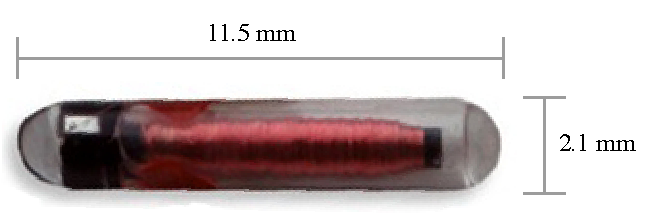
\includegraphics[width=0.5\textwidth]{assets/pdf/transponder.pdf}
  		\caption[Trovan ID-100A Microtransponder]{Pictured an ID-100A Microtransponder from $Trovan^{\copyright}$. The transponder weighs 0.1 g and the coat is made of biocompatible glass.\footnotesize Picture courtesy of Trovan.}
  		\label{fig:transponder}
\end{center}
\end{figure}
\begin{figure}[htpb]
\begin{center}
		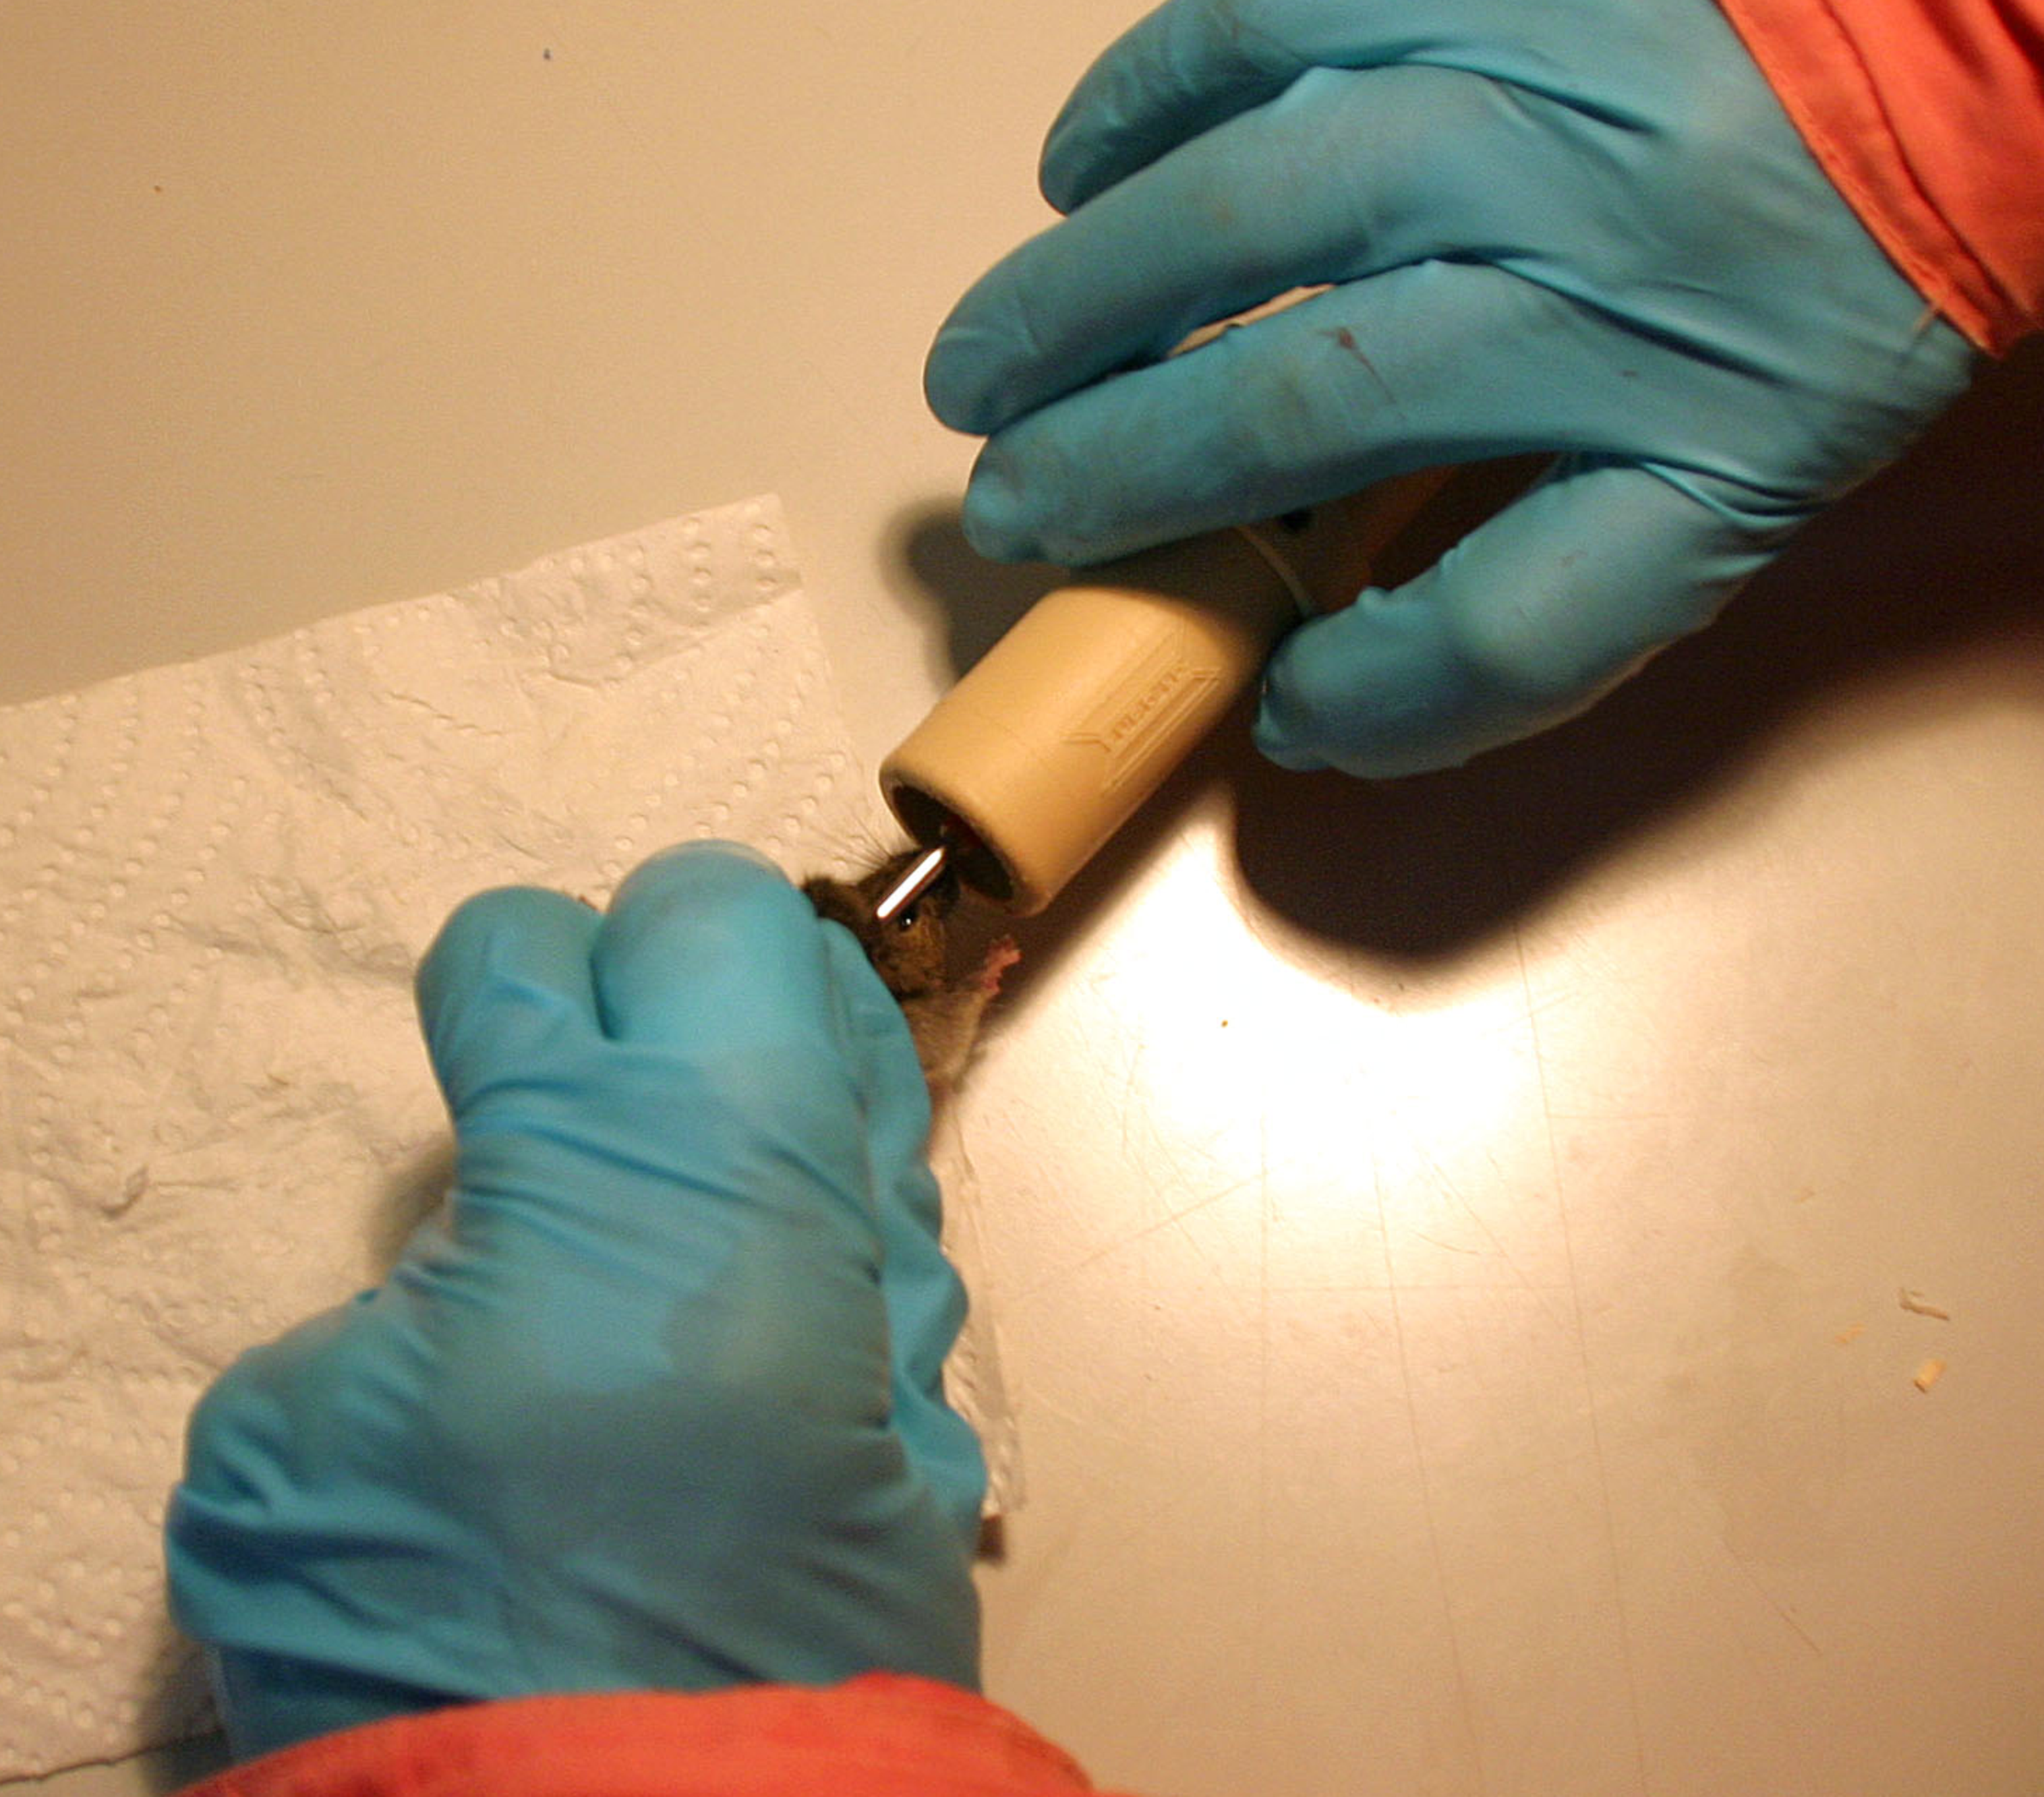
\includegraphics[width=0.5\textwidth]{assets/pdf/transponder_inject.pdf}
  		\caption[Injecting an RFID transponder]{Subcutaneous injection of an RFID transponder.}
  		\label{fig:inject_rfid}
\end{center}
\end{figure}

Furthermore, tissue samples are taken from the ear of each individual for genetic analysis. The genetical information provides an insight into the relatednesses within the mice population and allows to compare specific genetic markers. Genotypical information is not included in the data used for this thesis.

%----------------------------------------------
%Position / Time data
% ----------------------------------------------
\subsection{Collecting spatial position data}
\label{subsec:collectspatialpos}

To collect the spatial position data, a project specific system has been by built by \textit{New Behaviour}, a company specialized in developing technical systems to study animal behavior. 

The basic idea is to identify mice carrying an RFID transponder at specific locations. The locations where the identification occurs are the 40 artifical nestboxes distributed in the barn. 

An artificial nestbox consists of a cylinder, made of \ac{PVC}, with a diameter and a height of 15 centimeters and an entry tube made of \textit{Plexiglas} which is about 20 to 25 centimeters long. Wrapped around the tube are two antennas with a coverage area of 10 to 12 centimeters, capable of reading out the rfid transponders. Each antenna can be identified by an adress which is set manually. To improve the antenna accuracy, the entry tube is bent by 45 degrees to slow down the mice passing through. . Figure \ref{fig:artNestbox} depicts a model of such an artificial nestbox.
 
\begin{figure}[htbp]	
\centering	
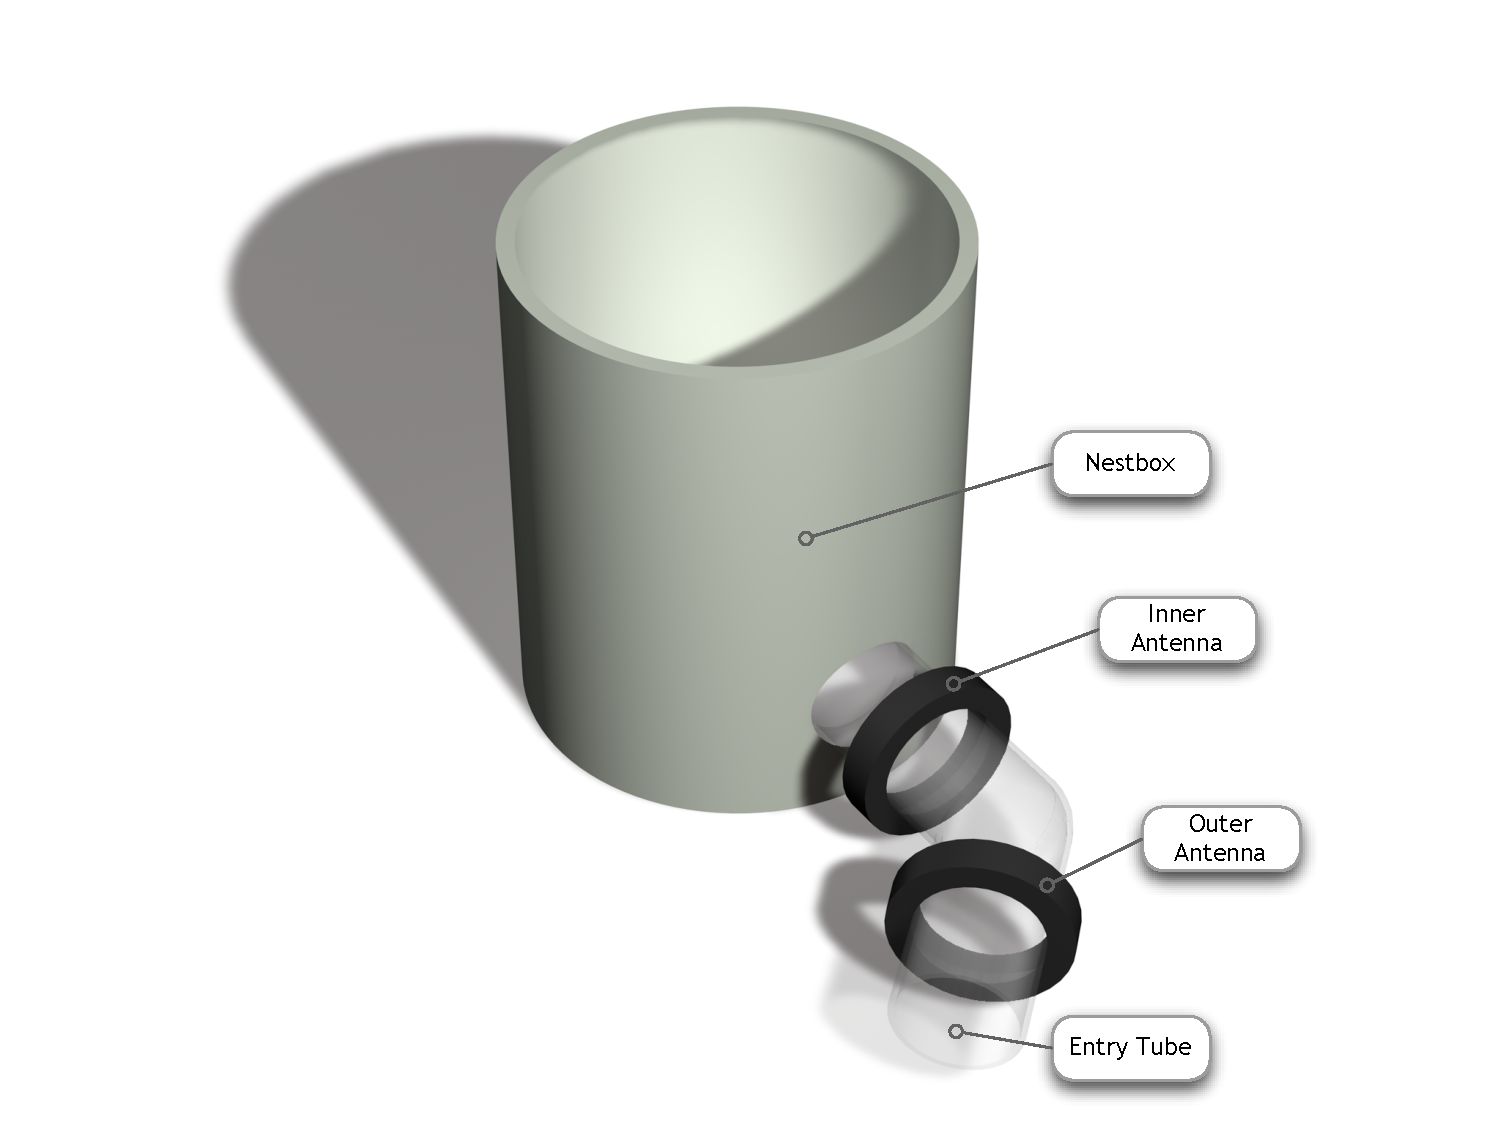
\includegraphics[width=0.75\textwidth]{assets/pdf/box_schema.pdf}	
\caption[Model of an artificial nestbox]{3d-Model of an artificial nestbox with the two antennas wrapped around the entry tube.}
\label{fig:artNestbox}
\end{figure}

The RFID transponders used are passive, meaning that they do not include a battery. The antenna acts as a scanner, presenting an inductive field which excites the transponder when entering the coverage area of the antenna. This energy is used by the transponder to send its identification to the antenna. 

So, whenever a mouse carrying a transponder passes by an antenna, it's identification is recorded and sent to a central computer along with the antenna address. The computer then adds a time value to the received data before writing it to a text file. The structure of these text files containing the data is explained in detail in the next section.

\subsubsection{Data file format}
\label{subsubsec:datafileformat}
The data files are simple text files, where each line denotes an event registered by an antenna in the system. Every day the data file is saved, closed, and a new one is created automatically by the system.

Basically there are to types of events. The first type occurs if the antenna could identify a transponder. In such a case a line as shown in figure \ref{fig:dataset} is written to the data file. The id of the transponder is a unique, ten character wide, alphanumeric value.

\begin{figure}[htbp]	
\centering	
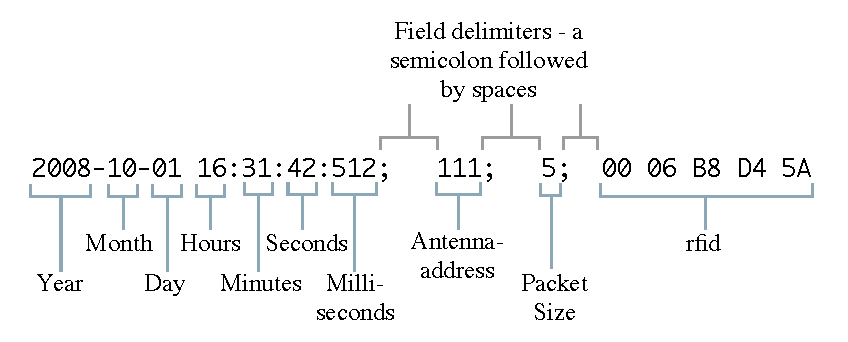
\includegraphics[width=0.75\textwidth]{assets/pdf/dataset.pdf}	
\caption[Dataset including an RFID transponder identification]{Typical dataset in a data file including an \ac{RFID} transponder identification}
\label{fig:dataset}
\end{figure}

The second type of event, for which the resulting data line looks like shown in figure \ref{fig:dataset_no_data}, occurs when a transponder enters or leaves the coverage area of an antenna.

\begin{figure}[htbp]	
\centering	
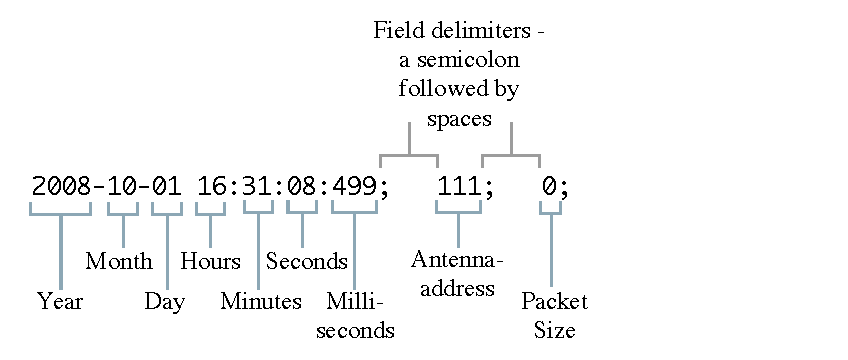
\includegraphics[width=0.75\textwidth]{assets/pdf/dataset_no_data.pdf}	
\caption[Dataset without RFID transponder identification]{Typical dataset in a data file without an \ac{RFID} transponder identification}
\label{fig:dataset_no_data}
\end{figure}

The following clipping and corresponding list show and explain the lines written to a data file, when a transponder passes by the two antennas beloning to an artificial nestbox. According to the previous explanations, the events are explained in the subsequent list.  

\numcodestyle
\begin{lstlisting}[frame=none]
2008-10-01 16:31:08:499;   111;   0; 
2008-10-01 16:31:09:095;   113;   0; 
2008-10-01 16:31:42:512;   111;   5;  00 06 B8 D4 5A
2008-10-01 16:31:42:807;   113;   5;  00 06 B8 D4 5A
2008-10-01 16:31:43:619;   111;   0; 
2008-10-01 16:31:44:014;   113;   0;
\end{lstlisting}

The list numbering matches the line numbering of the clipping.  

\begin{condensed_enum}
  \item Transponder \textbf{enters coverage area} of the antenna with address \lstinline|111|.
  \item Transponder \textbf{enters coverage area} of the antenna with address \lstinline|113|.
  \item Transponder is \textbf{identified} as \lstinline|00 06 B8 D4 5A| at antenna with address \lstinline|111|.
  \item Transponder is \textbf{identified} as \lstinline|00 06 B8 D4 5A| at antenna with address \lstinline|113|.
  \item Transponder \textbf{leaves coverage area} of the antenna with address \lstinline|111|.
  \item Transponder \textbf{leaves coverage area} of the antenna with address \lstinline|113|. 
\end{condensed_enum}
 
Depending on the event type, the value of the packet size is either a \lstinline|0|, for events without a transponder identification value, or a \lstinline|5| if the transponder has been identified. For the data processing (see section \ref{sec:dataproc} on page \pageref{sec:dataproc}) only the datasets with a transponder identification are taken into account.

\subsubsection{Antenna addressing}
\label{subsubsec:addressing}

The antenna address is three digits long, composed by the box number it is attached to (first two digits), and the position at the entry tube of the box. Outer antennas have a \lstinline|1| as the last digit of the address, inner antennas a \lstinline|3| (e.g the antennas attached to box 11 are addressed 111 for the outer, 113 for the inner antenna, respectively). Needless to say, that box numbers have to be unique.

Unfortunately there are a few exceptions to that schema, as for a few antennas, the correct addressing failed due to technical problems (see section \ref{subsec:problems}).

% \subsubsection{General system design and functionality}
% \label{subsubsec:generalsystem}
% 
% \begin{itemize}
%   \item Can-Bus
%   \item cable loop
%   \item rfid identification how
%   \item What happens in the boxes (boards) next to the antennas
%   \item How is can bus working/implemented
%   \item Where are the different cable loops (which antennas connected to a loop)
%   \item General system layout (cabling, protocols)
%   \item Programmed software
%   \item etc. 
% \end{itemize}

% ----------------------------------------------
%Data attributes
% ----------------------------------------------
\subsection{Collecting Data Attributes}
\label{subsec:dataattr}

During the \textit{population checks}, the whole barn, including all artificial nestboxes, plastic pipes and other structuring elements, is checked to collect attribute data of th emice according to the following procedure.

\begin{enumerate} 
	\item Each box is opened and the following observations made:
	\begin{mylist}
      \item \textbf{Mice in the box:} If adult mice are in the box, they get identified by their transponder, measured and weighed. Furthermore it will be checked, if the sex of the mouse has already been determined.  
      \item \textbf{Bedding:} Determine if the nestbox shows marks of usage, like trampled bedding.
      \item \textbf{Nest:} Determine wether the nestbox contains an open or closed nest built by the mice out of haw or straw regularly provided in the barn.  
      \item \textbf{Pups:} Does the box contain pups, and if yes how many and whats their estimated age. 
      \item \textbf{Communal nest:} Check if two or more litters are reared in the box. 
    \end{mylist}
	\item All the possible shelters, like planks an pipes, are checked for mice presence as well.
\end{enumerate}

% ----------------------------------------------
%storing Data
% ----------------------------------------------
\subsection{Data storage}
\label{subsec:datastorage}

This section contains detailed information about the design of the database. However, it is not designed as a documentation for computer scientists. Rather, it should reveal information contained in the database to researchers interested in the data.   

The data is stored in a \textit{MySQL}\footnote{\href{http://www.mysql.com/}{MySQL database}} database, which is  a \acf{RDBMS} (RDMS). Figure \ref{fig:database_schema} on page \pageref{fig:database_schema} in the appendix shows an overview of all the tables, including the data types\footnote{An overview of the MySQL data types can be found on the following webpage: \url{http://dev.mysql.com/doc/refman/5.0/en/data-types.html}} of the columns and their relations to columns in other tables.

Upon completion of a cascade of \ac{perl} scripts, which process and extract information from the spatial position data in the data files, the resulting data is merged with the collected attribute data and is written to the tables as outlined in this section. For details about the cascade refer to section \ref{sec:dataproc}. 

The tables can be split up in three different groups, depending of the sort of data they contain. 

\subsubsection{Processed data}
 
This group comprehends of the tables exclusively written to by the scripts in the import cascade. A schema of the tables belonging to that group, as well as the relations between them, is shown in figure \ref{fig:processed_data_schema}. 
 
\begin{figure}[htpb]
\begin{center}
  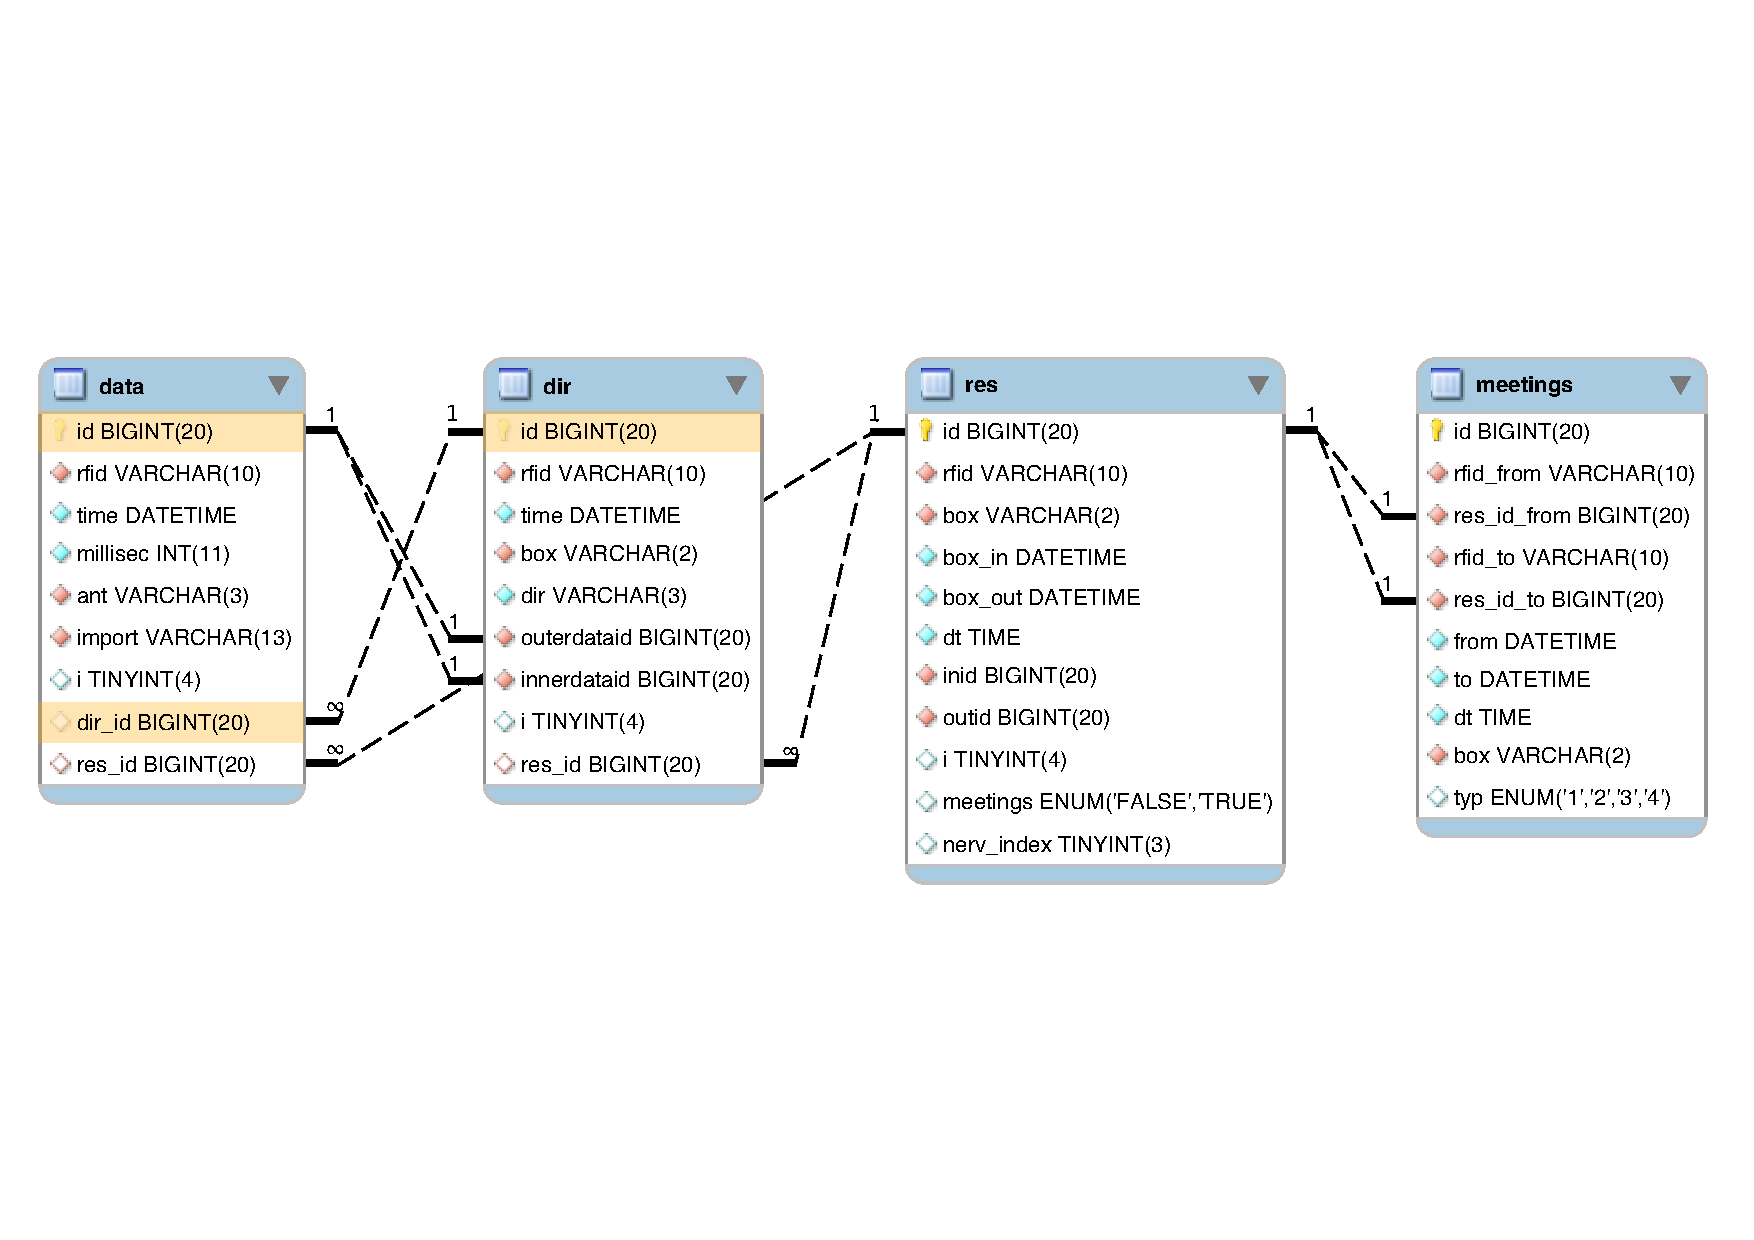
\includegraphics[width=\textwidth]{assets/pdf/processed_data_schema.pdf}
  \caption[Schema of database tables with processed data]{Schema of the database tables with the processed spatial position data and the relations between them.}
  \label{fig:processed_data_schema}
\end{center}
\end{figure} 

\paragraph{data table}
\label{para:data_table}

A script (see section \ref{subsec:importing}) imports the data files written by the antenna system in the barn into the \lstinline|data| table.

Shown next is a row of the \lstinline|data| table followed by short explanation of the columns.

\codescript
\begin{lstlisting}[frame=none]

(first part of table row)
+---------+------------+---------------------+----------+
| id      | rfid       | time                | millisec |
+---------+------------+---------------------+----------+
| 7321019 | 00069B4D4D | 2009-02-07 00:51:56 |      173 |
+---------+------------+---------------------+----------+

(second part of table row)
+-----+---------------+------+--------+--------+
| ant | import        | i    | dir_id | res_id |
+-----+---------------+------+--------+--------+
| 121 | 09-0206155809 |    4 |  40102 |  10001 |
+-----+---------------+------+--------+--------+

\end{lstlisting}

\begin{mydesc}
  \item \lstinline|id| is a unique identifier of a dataset in this table. Such a unique identifier is normally used as target for a relation between columns of different tables and does not have any further meaning.
  \item \lstinline|rfid| is a transponder value. This value is a reference to a value in the \lstinline|id| column of the \lstinline|rfid| table (see paragraph \ref{para:rfid_table}).
  \item \lstinline|time| and \lstinline|millsec| columns harbor the time the dataset has been recorded. Unfortunately the \textit{MySQL} \lstinline|DATETIME| data type does not include the milliseconds. Hence, these values have to be stored in a separate column.
  \item \lstinline|ant| denotes the antenna the data was recorded at. This value is a reference to a value in the \lstinline|id| column of the \lstinline|ant| table (see paragraph \ref{para:ant_table}.
  \item \lstinline|import| is a reference to a dataset in the \lstinline|logs| table, simply unveils of which data file this dataset is part of.
  \item \lstinline|i| is an indicator if the dataset could be used in a \lstinline|direction result| and \lstinline|stay result| (see \ref{para:res_table}). Table \ref{tab:i_values} on page \pageref{tab:i_values} of the appendix gives an overview of the meaning of the \lstinline|i| values in the different tables.
  \item \lstinline|dir_id| is a reference to an \lstinline|id| in the \lstinline|dir| table, if that dataset could be used in a \textit{direction result}. Else, this value is \lstinline|NULL|.
  \item \lstinline|res_id| is a reference to an \lstinline|id| in the \lstinline|res| table, if that dataset could be used in \textit{stay result}. Else this value is \lstinline|NULL|\footnote{\textit{MySQL} sets the \lstinline|NULL| value to indicate a missing or unknown value.}.
\end{mydesc}

\paragraph{dir table}
\label{para:dir_table}

Another script (see section \ref{subsec:dirres}) searches for matching pairs of datasets in the \lstinline|data| table which form a \textit{direction result}. When a mouse carrying a transponder passes the two antennas attached to the antry tube of an artificial nestbox, within a certain time, it is possible to determine if the mouse went in or out of that box. 

Shown next is a row of the \lstinline|dir| table followed by a short explanation of the columns.

\codescript
\begin{lstlisting}[frame=none]

(first part of table row)
+-------+------------+---------------------+-----+-----+
| id    | rfid       | time                | box | dir |
+-------+------------+---------------------+-----+-----+
| 40102 | 00069B4D4D | 2009-02-07 00:51:56 | 12  | in  |
+-------+------------+---------------------+-----+-----+

(second part of table row)
+-------------+-------------+------+--------+
| outerdataid | innerdataid | i    | res_id |
+-------------+-------------+------+--------+
|     7321019 |     7321020 |    4 |  10001 | 
+-------------+-------------+------+--------+
\end{lstlisting}

\begin{mydesc}
  \item \lstinline|id| and \lstinline|rfid| have the identical function as in the \lstinline|data| table.
  \item \lstinline|time| denotes the moment the the \lstinline|rfid| entered or left the \lstinline|box|.
  \item \lstinline|box| is a reference to a value in the \lstinline|id| column of the \lstinline|box| table (see paragraph \ref{para:box_table} on page \pageref{para:box_table}).
  \item \lstinline|dir| is either set to \lstinline|in| or \lstinline|out| and depicts the direction.
  \item \lstinline|outerdataid| and \lstinline|innerdataid| values can be used to backtrack the datasets in the \lstinline|data| table making up the \textit{direction result}. This is explained in detail in section \ref{subsec:dirres} on page \pageref{subsec:dirres}.
  \item \lstinline|i| is an indicator if the direction result could is used in a \textit{stay result} (see \ref{para:res_table}). Table \ref{tab:i_values} on page \pageref{tab:i_values} of the appendix gives an overview of the meaning of the \lstinline|i| values in the different tables.
  \item \lstinline|res_id| is a reference to an \lstinline|id| in the \lstinline|res| table, if that dataset could be used in \textit{stay result}. Else this value is \lstinline|NULL|.
\end{mydesc}

\paragraph{res table}
\label{para:res_table}

When two \textit{direction results}, one with a \lstinline|dir| value of \lstinline|in| and the other with a \lstinline|dir| value of \lstinline|out|, as well as matching \lstinline|rfid| and \lstinline|box| values are found, they form a so called \textit{stay result}.

Shown next is a row of the \lstinline|res| table followed by a short explanation of the columns.

\codescript
\begin{lstlisting}[frame=none]

(first part of table row)
+-------+------------+-----+---------------------+---------------------+----------+
| id    | rfid       | box | box_in              | box_out             | dt       |
+-------+------------+-----+---------------------+---------------------+----------+
| 10001 | 00069B4D4D | 12  | 2009-02-07 00:51:56 | 2009-02-07 00:52:01 | 00:00:05 |
+-------+------------+-----+---------------------+---------------------+----------+

(second part of table row)
+----------+-------+---------+------+----------+------------+
| dt       | inid  | outid   | i    | meetings | nerv_index |
+----------+-------+---------+------+----------+------------+
| 00:00:05 | 40102 | 7321021 |    4 | TRUE     |          1 | 
+----------+-------+---------+------+----------+------------+

\end{lstlisting}

\begin{mydesc}
	\item \lstinline|id|, \lstinline|rfid| and \lstinline|box| were already explained for the previous tables, and have the same function in this table.
	\item \lstinline|box_in| and \lstinline|box_out| denote the beginning and the end time of the stay of the \lstinline|rfid| in a \lstinline|box|.
	 \item \lstinline|inid| and \lstinline|outid| can be used to backtrace the datasets in the \lstinline|dir| or \lstinline|data| table making up the \textit{stay result}.
	 \item \lstinline|i| is either \lstinline|3| or \lstinline|4| and indicates the type of the result.
	 \item \lstinline|meetings| is set to \lstinline|true| when the result set has been analyzed for meetings (see next paragraph and section \ref{subsec:meetingres} for details about the \textit{meeting results}).
	 \item \lstinline|nerv_index| gives an idea about how \textit{nervous} the mouse was when she stayed in the box. 
\end{mydesc}

For detailed information about the meanings and formation of the columns, refer to section \ref{subsec:stayres}.

\paragraph{meetings table}
\label{para:meetings_table}

In this work, an event is termed a \textit{meeting}, if \textit{stay results} of different mice in the same box show a temporal overlap. The meeting data is written to the \lstinline|meeting| table (see section \ref{subsec:meetingres} on page \pageref{subsec:meetingres} for details).

Shown next is a row of the \lstinline|meetings| table followed by a short explanation of the columns.
\codescript
\begin{lstlisting}[frame=none]

(first part of table row)
++--------+------------+-------------+------------+-----------+
| id     | rfid_from  | res_id_from | rfid_to    | res_id_to |
+--------+------------+-------------+------------+-----------+
| 302635 | 0006CD478F |      596630 | 0006CC7962 |    596100 | 
+--------+------------+-------------+------------+-----------+

(second part of table row)
+---------------------+---------------------+----------+-----+------+
| from                | to                  | dt       | box | typ  |
+---------------------+---------------------+----------+-----+------+
| 2009-03-27 16:58:36 | 2009-03-27 17:01:00 | 00:02:24 | 13  | 1    |
+---------------------+---------------------+----------+-----+------+
\end{lstlisting}

\begin{mydesc}
	\item \lstinline|id| is again the unique identifier.
	\item \lstinline|rfid_from| and \lstinline|rfid_to| denote the two participating RFID's (mice) of the \textit{meeting result}.
	\item \lstinline|res_id_from| points to the \lstinline|id| of the \textit{stay result} from the \lstinline|rfid_from|, and the \lstinline|res_id_to| to the one of the \lstinline|rfid_to|. This allows to look up the the \textit{stay results} making up this \lstinline|meeting result|.
	\item \lstinline|from|, \lstinline|to| and \lstinline|dt| declare the start, the end time and the duration of the meeting.
	\item \lstinline|box| contains the reference to an \lstinline|id| in the \lstinline|box| table (see section \ref{para:box_table}).
	\item The different values of the \lstinline|typ| column are explained in detail in section \ref{subsec:meetingres}.
\end{mydesc}

\subsubsection{System members data}

This group encloses the tables which contain information about the rfids (transpondered mice) as well as the antennas and boxes.

Figure \ref{fig:system_members} shows an overview of the tables within this group plus the relations between the table columns. 

\begin{figure}[htpb]
\begin{center}
  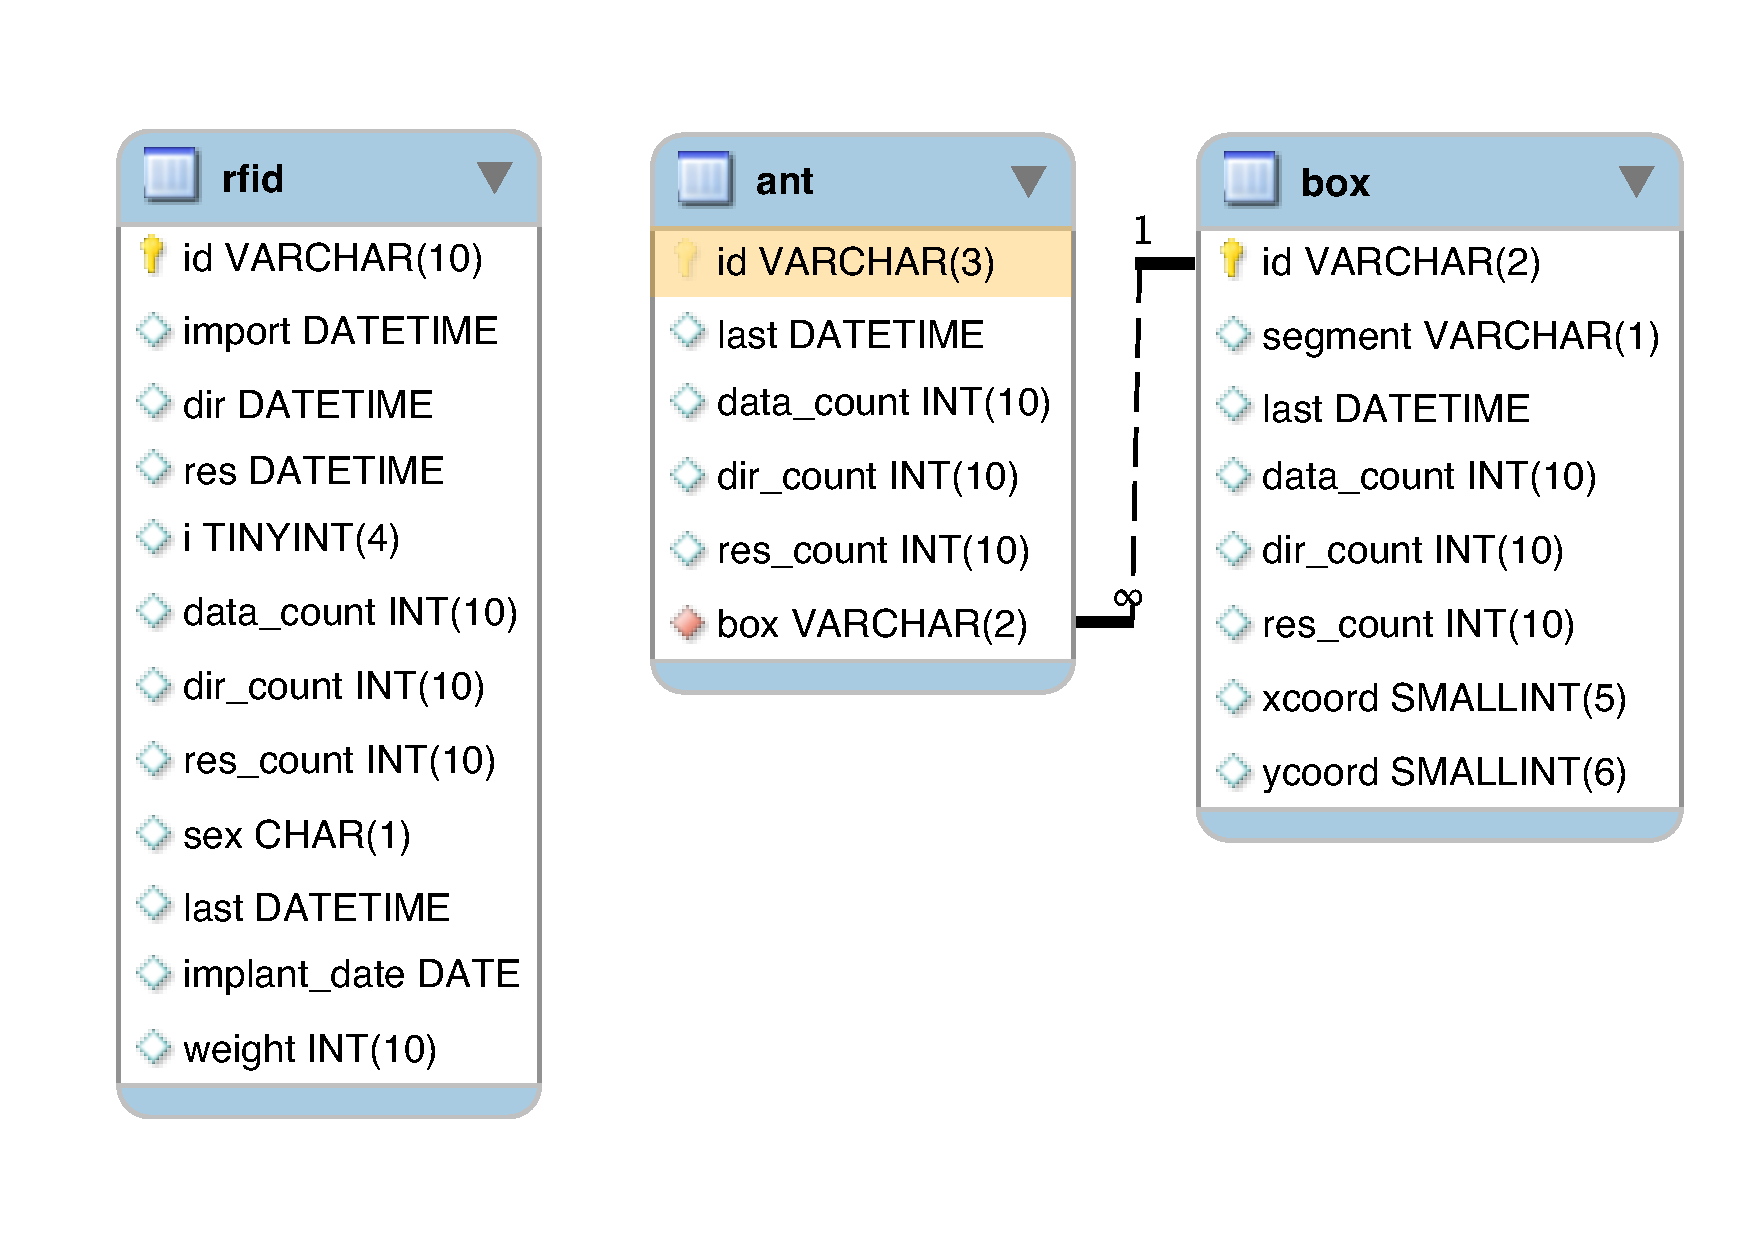
\includegraphics[width=0.75\textwidth]{assets/pdf/system_members_schema.pdf}
  \caption[Schema of database tables with system member data]{Schema of the database tables containing the \textit{system members} data.}
  \label{fig:system_members}
\end{center}
\end{figure}

\paragraph{rfid table}
\label{para:rfid_table}

All the rfids ever recorded by the system, including their corresponding attribute data are stored in the  \lstinline|rfid| table.

Shown next is a row of the \lstinline|rfid| table followed by short a explanation of the columns.
\codescript
\begin{lstlisting}[frame=none]

(first part of table row)
+------------+------+------------+-----------+-----------+
| id         | i    | data_count | dir_count | res_count |
+------------+------+------------+-----------+-----------+
| 0006955EED |    3 |          1 |         0 |         0 |
+------------+------+------------+-----------+-----------+

(second part of table row)
+------+---------------------+--------------+--------+
| sex  | last                | implant_date | weight |
+------+---------------------+--------------+--------+
| m    | 2007-08-29 23:35:41 | 2007-08-28   |   18.0 |
+------+---------------------+--------------+--------+

\end{lstlisting}

\begin{mydesc}
	\item \lstinline|id| is the unique, 10 character wide alphanumeric transponder identification.
	\item \lstinline|i| is is a helper value used in the data import procedure. It is \lstinline|0| if new data for the transponder has been imported, \lstinline|2| if the data is searched for \textit{direction results} and \lstinline|3| if the data has been searched for \textit{stay results} .
	\item \lstinline|data_count| contains the sum of datasets in the \lstinline|data| table.
	\item \lstinline|dir_count| contains the sum of datasets in the \lstinline|direction| table.
	\item \lstinline|res_count| contains the sum of datasets in the \lstinline|results| table.
	\item \lstinline|sex| denotes the gender of the mouse, if it is known.
	\item \lstinline|last| points to the maximum value in the \lstinline|time| column of the \lstinline|data| table for this mouse, which is just the last time the transponder has been recorded by the antenna system.
	\item \lstinline|implant_date| holds the date of the transponder injection.
	\item \lstinline|weight| contains a decimal number with the weight of the mouse in grams.
\end{mydesc}

\paragraph{box table}
\label{para:box_table}

The box table contains all the information about the 40 artificial nestboxes. 

Shown next is a row of the \lstinline|box| table followed by a short explanation of the columns.
\codescript
\begin{lstlisting}[frame=none]

(first part of table row)
+----+---------+---------------------+------------+
| id | segment | last                | data_count |
+----+---------+---------------------+------------+
| 01 | A       | 2009-03-27 16:38:59 |     122439 | 
+----+---------+---------------------+------------+

(second part of table row)
+-----------+-----------+--------+--------+
| dir_count | res_count | xcoord | ycoord |
+-----------+-----------+--------+--------+
|     44389 |      9824 |    246 |    708 | 
+-----------+-----------+--------+--------+

\end{lstlisting}

\begin{mydesc}
	\item \lstinline|id| is the unique 2 character wide box identification.
	\item \lstinline|segment| points to the segment (A, B, C or D) the box is located in.
	\item The meaning of the \lstinline|last| \lstinline|data_count|, \lstinline|dir_count| and \lstinline|res_count| columns was already explained in the \lstinline|rfid| table.
	\item \lstinline|xcoord| and \lstinline|ycoord| denote the position of the nestbox in the barn. The entrance wall stands for the x-axis, the side wall to the left of the entrance for the y-axis of the coordinate system. The coordinate values are stored in centimeters. 
\end{mydesc}

\paragraph{ant table}
\label{para:ant_table}

The ant table contains all the information about the 80 antennas. 

Shown next is a row of the \lstinline|ant| table followed by a short explanation of the columns.
\codescript
\begin{lstlisting}[frame=none]
+-----+---------------------+------------+-----------+-----------+-----+
| id  | last                | data_count | dir_count | res_count | box |
+-----+---------------------+------------+-----------+-----------+-----+
| 011 | 2009-03-27 16:38:59 |      54220 |     46099 |     19648 | 01  | 
+-----+---------------------+------------+-----------+-----------+-----+

\end{lstlisting}

\begin{mydesc}
	\item \lstinline|id| is the unique 3 character wide antenna identification.
	\item The meaning of the \lstinline|last| \lstinline|data_count|, \lstinline|dir_count| and \lstinline|res_count| columns was already explained in the \lstinline|rfid| table.
	\item \lstinline|box| points to the \lstinline|id| value in the \lstinline|box| table, the antenna is attached to.
\end{mydesc}

\subsubsection{Auxiliary tables}

Tables in this group contain data about the imported data files, and precalculated values to improve the performance when browsing the data using the graphical user interface.

Figure \ref{fig:auxiliary_tables} shows an overview of the tables within this group. 


\begin{figure}[htpb]
\begin{center}
  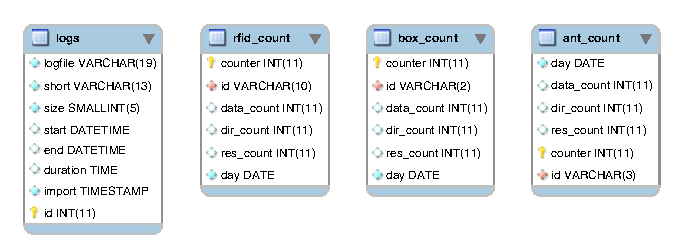
\includegraphics[width=0.75\textwidth]{assets/pdf/auxiliary_tables_schema.pdf}
  \caption[Schema of database tables with system member data]{Schemata of the database tables with the auxiliary data. The relations are not shown.}
  \label{fig:auxiliary_tables}
\end{center}
\end{figure}

\paragraph{logs table}
\label{para:logs_table} 

The \lstinline|logs| table contains information about the imported data files.

Shown next is a row of the \lstinline|logs| table followed by a short explanation of the columns.

\codescript
\begin{lstlisting}[frame=none]
(first part of table row)
+-----+---------------------+---------------+------+---------------------+
| id  | logfile             | short         | size | start               |
+-----+---------------------+---------------+------+---------------------+
| 608 | 20090326_170750.txt | 09-0326170750 | 1660 | 2009-03-26 17:07:51 |
+-----+---------------------+---------------+------+---------------------+

(second part of table row)
+---------------------+----------+---------------------+
| end                 | duration | import              |
+---------------------+----------+---------------------+
| 2009-03-27 17:07:40 | 23:59:49 | 2009-04-12 01:03:01 | 
+---------------------+----------+---------------------+

\end{lstlisting}

\begin{mydesc}
	\item \lstinline|id| is the unique identifier of dataset.
	\item The original filename of the data file is stored in the \lstinline|logfile| column.
	\item \lstinline|short| values are a kind of code made up from parts of the data filename. This column was important at the beginning of the project, when we had to import data files with a another format.
	\item \lstinline|size| contains the filesize in bytes of the data file.
	\item \lstinline|start| and \lstinline|end| indicate the first and last point in time of an antenna reading, this data file contains.
	\item \lstinline|duration| is simply the period between the \lstinline|start| and \lstinline|end| values.
	\item \lstinline|import| refers to the time the import of the data in the file into the \lstinline|data| table has been finished.
\end{mydesc}

\paragraph{rfid\_count, box\_count, ant\_count}
\label{para:counts}

These three tables contains the per day data counts for transponders (\lstinline|rfid_count|), boxes (\lstinline|box_count|) and antennas (\lstinline|ant_count|), and are exclusively needed by the user interface to allow faster browsing of the data.

Shown next is a row of the \lstinline|rfid_count|, \lstinline|box_count|, \lstinline|ant_count| tables followed by a short explanation of the columns.

\codescript
\begin{lstlisting}[frame=none]
(row of table rfid_count)
+---------+------------+------------+------------+-----------+-----------+
| counter | id         | day        | data_count | dir_count | res_count |
+---------+------------+------------+------------+-----------+-----------+
|     999 | 0006B9C5E8 | 2008-07-14 |         10 |         4 |         2 | 
+---------+------------+------------+------------+-----------+-----------+


(row of table box_count)
+---------+----+------------+------------+-----------+-----------+
| counter | id | day        | data_count | dir_count | res_count |
+---------+----+------------+------------+-----------+-----------+
|     999 | 10 | 2008-07-31 |        259 |       114 |        39 | 
+---------+----+------------+------------+-----------+-----------+


(row of table ant_count)
+---------+-----+------------+------------+-----------+-----------+
| counter | id  | day        | data_count | dir_count | res_count |
+---------+-----+------------+------------+-----------+-----------+
|     999 | 121 | 2008-07-19 |        196 |       174 |        47 | 
+---------+-----+------------+------------+-----------+-----------+


\end{lstlisting}

\begin{mydesc}
	\item \lstinline|counter| is the unique identifier of dataset.
	\item \lstinline|id| contains the \lstinline|id| value of the transponder, the box or the antenna.
	\item \lstinline|day| points to the day the table row holds the data counts for.
	\item \lstinline|data_count|, \lstinline|dir_count| and \lstinline|res_count| contain the per day counts for the datasets, the \textit{direction results} and the \textit{stay results}.
\end{mydesc}

\subsection{Efficiency and problems of the antenna system}
\label{subsec:problems}

Unfortunately the problems with the antenna system are diverse. Antenna drop outs, broken laptop or cable connections chewed by the mice, to name just a few. Some of these problems could be solved, other still remain.

However, one of biggest problem is, that the readings at the antennas are not as reliable as planned. This is clearly visible by looking at the efficiency of the system.

From the 5 of April 2007 to the 27 of March 2009, 8,171,945 datasets (table \lstinline|data|) have been collected. Assuming that the system works perfect, we would get 4,085,972 \textit{direction results}. Compared to the real number of \textit{direction results}, which is 2,907,495 , we have a yield of 71.16\%.

In the next step, two \textit{direction results} should create a \textit{stay result}. The script which searches for the \textit{stay results} could find 1,453,747 results in the 2,907,495 \textit{direction results}, but finds 992,128 which is 68.25\%. Most likely these low numbers are an effect of missed antenna readings.

Normally, an antenna reads out the transponder information 10 times, to ensure maximum reliability of a correct reading. The antenna system in the barn, however, reads out the identification only 3 times, as the time that a transpondered mouse spends in the coverage area of an antenna is usually short. We are able to partially comprehend the impact of this factor by looking at the \lstinline|rfid| table. The table contains 4605 different transponder id's, whereof only 1014 have been read at an antenna more then 10 times. The other 3546 rfids are most probably a result a phenomeneon called \textit{bit flipping}.

The following listing shows a clipping of a data file, where a transponder is identified as \lstinline|00 05 B8 D2 70| on line two, but as \lstinline|00 06 B8 E2 70| on the other lines. 

\numcodestyle
\begin{lstlisting}[frame=none]
2007-11-25 10:09:12:906;   381;   5;  00 06 B8 E2 70
2007-11-25 10:09:16:529;   381;   5;  00 05 B8 D2 70
2007-11-25 10:09:16:932;   381;   5;  00 06 B8 E2 70
2007-11-25 10:09:19:950;   381;   0; 
2007-11-25 10:09:20:253;   381;   5;  00 06 B8 E2 70
\end{lstlisting}

The first four digits of the transponder identification represents some sort of the manufacturer series. The manufacturer sold only transponder from the \lstinline|00 06| series to us. Just out of this fact, we can conclude, that line two is a read error. Still, this transponder has been read 53 times between the November 2007 and May 2008, but none of the readings could be used to form a \textit{direction result}. Assuming that this is not a singular case, we get many of these false readings, leading to a low rate of yield in the following data processing. 

Furthermore, for some antennas, the address could not be set properly. In one case two antennas even sent the same address, so that distinction of the data is impossible. The workaround for this problem is to find an unused address which we are able to set, and map it to the desired address during the data import (see section \ref{subsec:importing} on page \pageref{subsec:importing}).   

\subsection{Data access}
\label{subsec:dataccess}

Most of the mainly used relational databases offer \ac{SQL} (SQL) to manage and retrieve the data. However, SQL is not easy to learn and use, lacks built-in export functionality to file formats such as \textit{Microsoft Excel}, and does not offer any possibility to visualize the data. Therefore, a feature rich but still handy and intuitive, \ac{GUI} (GUI) is available, making it easy for the user to explore, visualize and export data. A presentation to the GUI can be found in section \ref{sec:dataaccessandexp}.